\documentclass{beamer}

\mode<presentation> {
  \usetheme{PaloAlto}
}

%%
\makeatletter
\setbeamertemplate{subsubsection in sidebar}{\vspace*{-\baselineskip}}
\setbeamertemplate{subsubsection in sidebar shaded}{\vspace*{-\baselineskip}}
\makeatother
%%

%%
\setbeamertemplate{theorems}[numbered]
%%

\definecolor{Garnet}{RGB}{130,0,20}
\usecolortheme[named=Garnet]{structure}

\logo{
\includegraphics[width=1.5cm]{../../sharedImgs/USClogo.png}}

%\setbeamercolor{title}{fg=red!60!black,bg=white!50!black}
%\usecolortheme{beaver}
%\usecolortheme{crane}
\usefonttheme{structuresmallcapsserif}
\usefonttheme[onlysmall]{structurebold}

\usepackage{multicol}
\usepackage{graphicx}
\usepackage{mathtools}
\usepackage{latexsym}
\usepackage{amsfonts}
\usepackage[only,ninrm,elvrm,twlrm,sixrm,egtrm,tenrm]{rawfonts}
\usepackage{indentfirst}
\usepackage[noend]{algorithmic}
\usepackage{algorithm}
\usepackage{enumerate}
\usepackage{graphicx,psfrag}
\usepackage{epsfig}
%\usepackage[pdflatex]{graphicx}
%\usepackage{epstopdf}
\usepackage{ulem}
\usepackage{animate} %need the animate.sty file
\usepackage{tikz}
\usetikzlibrary{fit,shapes,calc}
\usepackage{pgfplots}
\usepackage{amsmath,amsthm,amssymb,amsfonts,enumerate,mymath,mathtools,tikz-cd,mathrsfs}

\newtheorem{thm}{Theorem}
\newtheorem{lem}{Lemma}
\newtheorem{prop}{Proposition}
\theoremstyle{definition}
\newtheorem{defn}{Definition}
\newtheorem{rmk}{Remark}

\newcommand{\A}{\mathscr{A}}
\renewcommand{\C}{\mathscr{C}}

\newcommand*{\defeq}{\mathrel{\vcenter{\baselineskip0.5ex \lineskiplimit0pt
                     \hbox{\scriptsize.}\hbox{\scriptsize.}}}%
                     =}
\DeclarePairedDelimiter\ceil{\lceil}{\rceil}
\DeclarePairedDelimiter\floor{\lfloor}{\rfloor}

\input epsf



\usepackage[english]{babel}
% or whatever

\usepackage[latin1]{inputenc}
% or whatever

\usepackage{times}
\usepackage[T1]{fontenc}
% Or whatever. Note that the encoding and the font should match. If T1
% does not look nice, try deleting the line with the fontenc.

\title % (optional, use only with long paper titles)
    {Proportionality and Power Functions}

\author[Farman]
{Blake Farman~\inst{1}}

\institute[USC]{
\inst{1}
University of South Carolina, Columbia, SC USA}
%\inst{2}
%East Carolina University, Greenville, NC USA\\
%\inst{3}
%University of Johannesburg, Auckland Park, South Africa}

\date[January 17, 2017]
{Math 122: Calculus for Business Administration and Social Sciences}

%\subject{Irredundant and Mixed Ramsey Numbers}
\setbeamercolor{alerted text}{fg=red!60!black}
\setbeamercolor{block title}{bg=white!50!black,fg=red!60!black}

\begin{document}

\begin{frame}
  \titlepage
\end{frame}

\begin{frame}
  \frametitle{Outline}
  \tableofcontents[pausesections]
\end{frame}

\section{2.1: Instantaneous Rate of Change}
\begin{frame}{Definition}
  The {\it instantaneous rate of change} of $f$ at $a$ is defined to be the limit of the average rates of change of $f$ over successively smaller intervals around $a$.
  This is also known as the {\it derivative of $f$ at $a$}.

\end{frame}

\begin{frame}{Example}
  The quadratic
  $$s(t) = -4.9t^2 + 9.8t$$
  models the position of an object thrown vertically into the air with an initial velocity of $9.8$ m/s.
  \onslide<2->{The graph of the quadratic is
    \begin{center}
      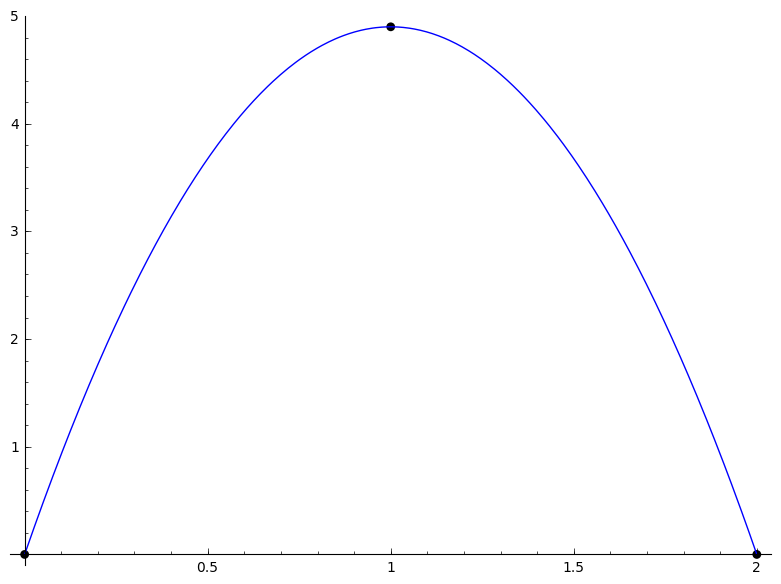
\includegraphics[scale=0.25]{imgs/kinematics.png}
  \end{center}}
  \onslide<3->{What is the instantaneous rate of change at the vertex, where $t = 1$?}
\end{frame}

\begin{frame}{Example (Cont.)}
  Here are some values:
  \begin{center}
    \begin{tabular}{ll}
      \onslide<1->{t & $\frac{f(t) - f(1)}{t - 1}$\\}
      \onslide<2->{0 & 4.9\\}
      \onslide<3->{0.9 & $\approx$ 0.49\\}
      \onslide<4->{0.99 & $\approx$ 0.049\\}
      \onslide<5->{0.999 & $\approx$ 0.0049\\}
      \onslide<6->{0.9999 & $\approx$ 0.00049\\}
      \onslide<7->{0.99999 & $\approx$ 0.000049\\}
      \onslide<8->{0.999999 & $\approx$ 0.0000049\\}
    \end{tabular}
  \end{center}
  \onslide<9->{So, we would guess that the instantaneous rate of change is 0 at $t = 1$.}
\end{frame}

\section{2.2: The Derivative Function}
\begin{frame}{Definition}
  \begin{defn}
    \begin{itemize}
    \item<1->
      If a function, $f$, has a derivative at every point in its domain, then we say that $f$ is {\it differentiable}.
    \item<2->
      In this case, we can define a function $f^\prime(x)$ that outputs the instantaneous rate of change of $f$ at $x$.
    \item<3->
    We call $f^\prime(x)$ the {\it derivative function}.
    \end{itemize}
  \end{defn}
\end{frame}

\begin{frame}{The Tangent Line}
  \begin{defn}
    \begin{itemize}
    \item<1->
      We can regard $f^\prime(x_0)$ as a velocity by viewing it as the slope of a line passing through $(x_0,f(x_0))$.
    \item<2->
      We call the line
      $$y - f(x_0) = f^\prime(x_0)(x - x_0)$$
      the {\it line tangent to $f$ at $(x_0, f(x_0))$}.
    \end{itemize}
  \end{defn}
\end{frame}

\begin{frame}{Linearization}
  \begin{itemize}
    \item<1->
      Since we defined $f^\prime(x_0)$ by a limit, 
      $$f^\prime(x_0) \approx \frac{f(x) - f(x_0)}{x - x_0}$$
      for $x$ close to $x_0$.
    \item<2->
      Writing $\Delta x = x - x_0$ we can get a good linear approximation of $f$ close to $x_0$:
      $$f(x) \approx f^\prime(x)\Delta x + f(x_0)$$
      called the {\it Tangent Line Approximation}.
    \item<3->
      This means $f$ locally looks like a line!
  \end{itemize}
\end{frame}

\begin{frame}{Non-Differentiable Function}
  Consider the absolute value function
  $$\abs{x} = \left\{\begin{array}{ll}x & \text{if}\ 0 \leq x,\\-x & \text{else}\end{array} \right.$$
  at the point $(0,0)$.
  \begin{itemize}
    \item<2->
      For all $x < 0$, 
      $$\frac{\abs{x} - 0}{x - 0} = \frac{-x}{x} = -1.$$
    \item<3->
      For all $0 < x$,
      $$\frac{\abs{x} - 0}{x - 0} = \frac{x}{x} = 1.$$
    \item<4->
      So the derivative at $(0,0)$ is {\bf not} defined: it's -1 if we approach from left to right, and 1 if right to left.
  \end{itemize}
\end{frame}

\begin{frame}
  What does the derivative tells us about the original function?
  On the interval $(a,b)$, if for all $a \leq x \leq b$
  \begin{itemize}
  \item<2->
    $f^\prime(x) \leq 0$, then $f$ is decreasing on $(a,b)$,
  \item<3->
    $0 \leq f^\prime(x)$, then $f$ is increasing on $(a,b)$,
  \item<4->
    $f^\prime(x) = 0$, then $f$ is constant on $(a,b)$.
  \end{itemize}
\end{frame}
\end{document}
